\FloatBarrier
\section{Aufgabe 1}
\label{sec:A1}
\textbf{Disclaimer:} Ich habe nicht mal ansatzweise eine Ahnung,
ob das, was wir gemacht haben richtig ist oder ob meine physikalische Interpretation nur Wunschdenken ist,
aber here goes nothing...
%\includegraphics{code/build/plot.pdf}
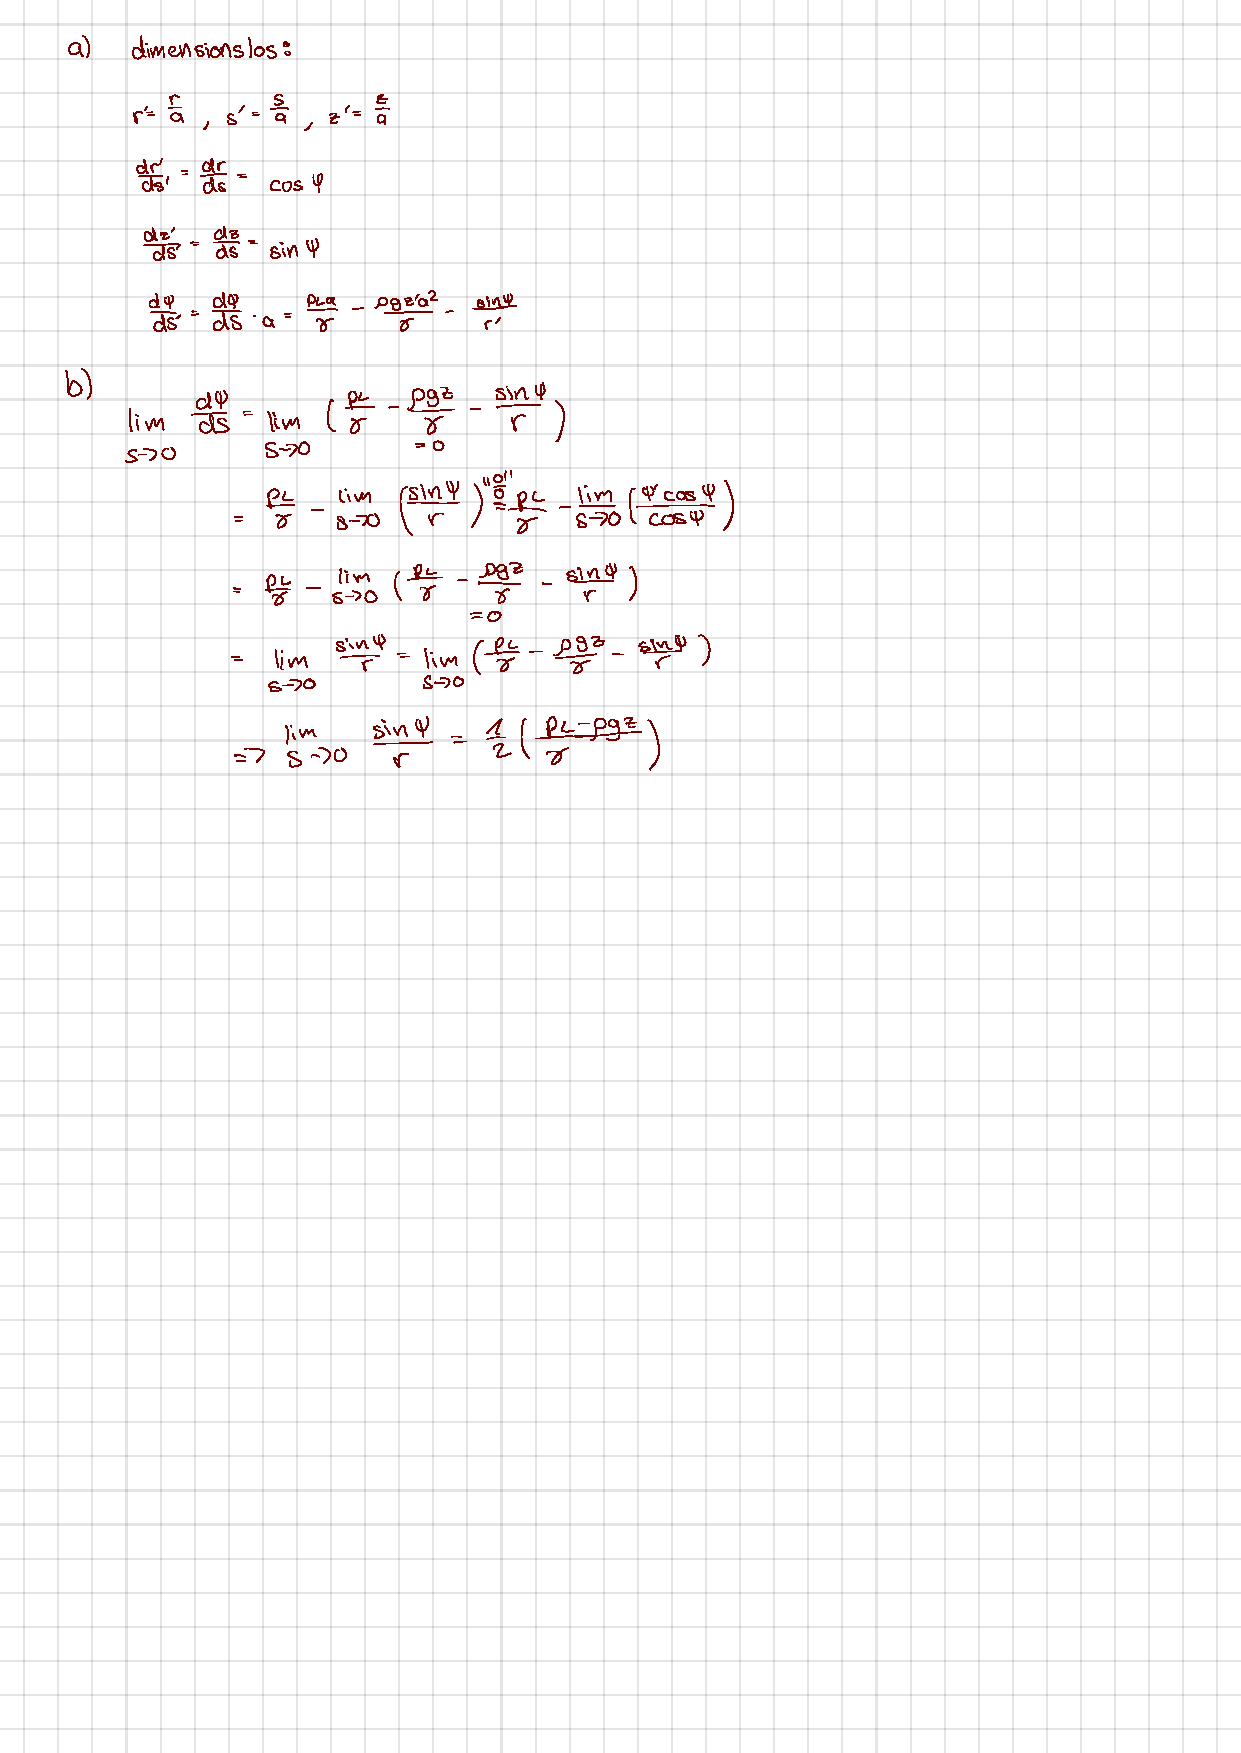
\includepdf[pages=-]{content/A1_ab.pdf}
\subsection*{c)}
Das Runge-Kutta-Verfahren:
\begin{equation*}
    \displaystyle y'(t)=f\left(t,y(t)\right),\quad y(t_{0})=y_{0},\quad y\colon \mathbb {R} \to \mathbb {R} ^{d}
\end{equation*}

\begin{equation*}
\displaystyle {\begin{aligned}k_{1}&=f(t_{i},y_{i}),\\
    k_{2}&=f(t_{i}+{\frac {h}{2}},y_{i}+{\frac {h}{2}}k_{1}),
    \\k_{3}&=f(t_{i}+{\frac {h}{2}},y_{i}+{\frac {h}{2}}k_{2}),
    \\k_{4}&=f(t_{i}+h,y_{i}+hk_{3}).\end{aligned}}
\end{equation*}

\begin{equation*}
\displaystyle y_{i+1}=y_{i}+h\cdot {\frac {1}{6}}\left(k_{1}+2k_{2}+2k_{3}+k_{4}\right),\quad i=0,1,\dots 
\end{equation*}

Für dieses Problem:
\begin{equation*}
     f = \begin{pmatrix}
        \frac{d r'}{S'} \\ 
        \frac{d z'}{S'} \\
        \frac{d \psi'}{S'} 
    \end{pmatrix}
\end{equation*}
Die Ableitung für $\frac{d \psi }{d S'}$ bei $r'(S'(0))=0$ ist gleich
\begin{equation*}
    \frac{d \psi }{d S'}= \frac{p_L a}{2 \gamma} - \frac{\rho g z' a^2}{2 \gamma} = (2-0,1 z') / 2.
\end{equation*}
Der Algorithmus wird bei dem dreifachen von $r=\tfrac{a}{2}$, also $r'= 3 \cdot \tfrac{1}{2}$ gestoppt.

\begin{figure}
    \centering
    \includegraphics[width=0.7\textwidth]{code/build/A1_r.pdf}
\end{figure}

\begin{figure}
    \centering
    \includegraphics[width=0.7\textwidth]{code/build/A1_z.pdf}
\end{figure}


\begin{figure}
    \centering
    \includegraphics[width=0.7\textwidth]{code/build/A1_psi.pdf}
\end{figure}

\subsection*{d)}
Also falls ich das richtig interpretiere, 
entspricht der erste Teil(mit der roten Linie abgestrennt) einer kompletten Formkurve
(also dem positiven Teil des Tropfens). 
Der Rest, der danach kommt ist einfach nur die wiederholte Berechnung der Formkurve.

Der Parameterraum ist dementsprecht die Wertermenge in dem ersten Teil:
\begin{equation*}
    \begin{aligned}
        r' &\in [0;1.01762]\\
        z' &\in [0;2.18968]\\
        \psi &\in [0;2.6015]\\
        S' &\in [0;0.0331]\\
    \end{aligned}
\end{equation*}
\FloatBarrier

Druck-Volumen-Kurve: Keine Ahnung.

